
\section{Анализ подходов к решению поставленной задачи}
\label{sec:domain1}

Для проекта SCn-редактор целью работы в данном семестре было:
\begin{enumerate}
\item{Реализовать возможность создания и редактирования ссылок;}
\item{Привести в соответствие правилам возможности редактирования основных идентификаторов;}
\item{Исправить проблему обновления корневого элемент контура;}
\item{Исправить ошибку при открытии SCg-редактора в SCn-статье;}
\item{Протестировать систему.}
\end{enumerate}

Для этого необходимо решить следующие задачи:
\begin{enumerate}
\item{Протестировать систему;}
\item{Устранить существующие проблемы;}
\item{Добавить новые возможности.}
\end{enumerate}

Для проекта SCg-интерфейс целью работы в данном семестре было:
\begin{enumerate}
\item{Реализовать создание gwf-файлов для KBE редактора;}
\item{Исправить проблему со скрытием информации с ссылок после перехода по истории;}
\item{Исправить проблему c невозможностью создания элементов после удаления всех элементов.;}
\item{Реализовать кнопку очистки всех объектов с рабочей области редактора и написать ее спецификацию;}
\item{Оптимизировать размер кнопок;}
\item{Добавить возможность загрузки изображений через SCg-редактор.}
\end{enumerate}

Для этого необходимо решить следующие задачи:
\begin{enumerate}
\item{Устранить существующие проблемы;}
\item{Добавить новые возможности.}
\end{enumerate}

Для проекта ИСС по Теории Графов целью работы в данном семестре было:
\begin{enumerate}
\item{Создать свой компонент для отображения и редактирования графов.}
\end{enumerate}

Для этого необходимо решить следующие задачи:
\begin{enumerate}
\item{Реализовать свой компонент на базе SCg;}
\item{Реализовать скрипты установки компонента;}
\item{Реализовать трансляцию элементов из редактора в SC-память;}
\item{Реализовать загрузку графа из SC-памяти в свой компонент;}
\item{Встроить SCs компонент в редактор;}
\item{Синхронизировать встроенный SCs компонент с редактором;}
\item{Обеспечить удобную и продуктивную работу с пользовательским интерфейсом.}
\end{enumerate}

\section{Личный вклад в развитие проекта ИСС по теории графов}
\label{sec:domain2}

\subsection{Реализация трансляции элементов из редактора в SC-память}

В рамках этого пункта, для первой версии редактора графов были выполнены следующие задачи:

\begin{enumerate}
\item{Изменена модель представления вершин;}
\item{Изменена модель представления ребер;}
\item{Изменена модель представления дуг;}
\item{Реализована форма ввода основного идентификатора графа;}
\item{Реализовано создание структуры графа с присвоением ему осинового идентификатора и системного идентификатора;}
\item{Реализована трансляция вершин из редактора в SC-память;}
\item{Реализована трансляция дуг из редактора в SC-память;}
\item{Реализована трансляция вершин из редактора в SC-память.}
\end{enumerate}

Демонстрация создания нового графа.

\begin{figure}[H]
  \centering
  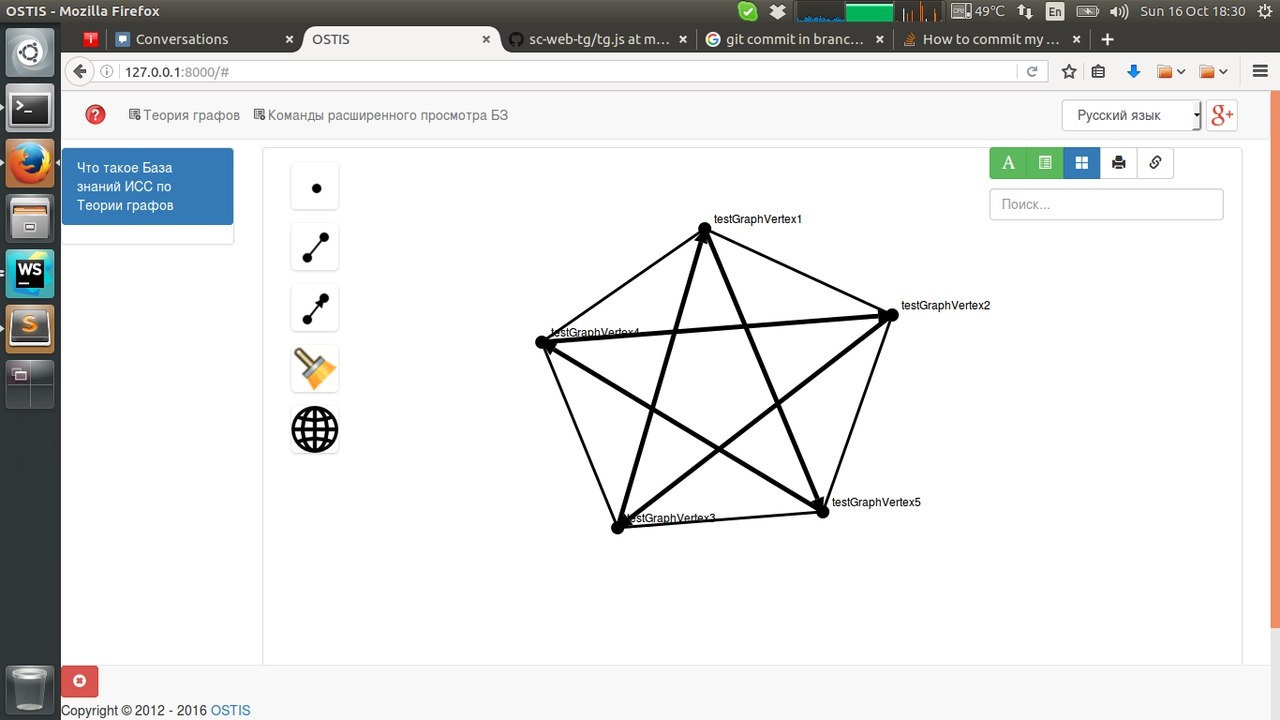
\includegraphics[width=\textwidth]{1.jpg}
  \caption{Первая версия редактора графов с введенным графом}
  \label{fig:hardware:sdr_pipeline}
\end{figure}

\begin{figure}[H]
  \centering
  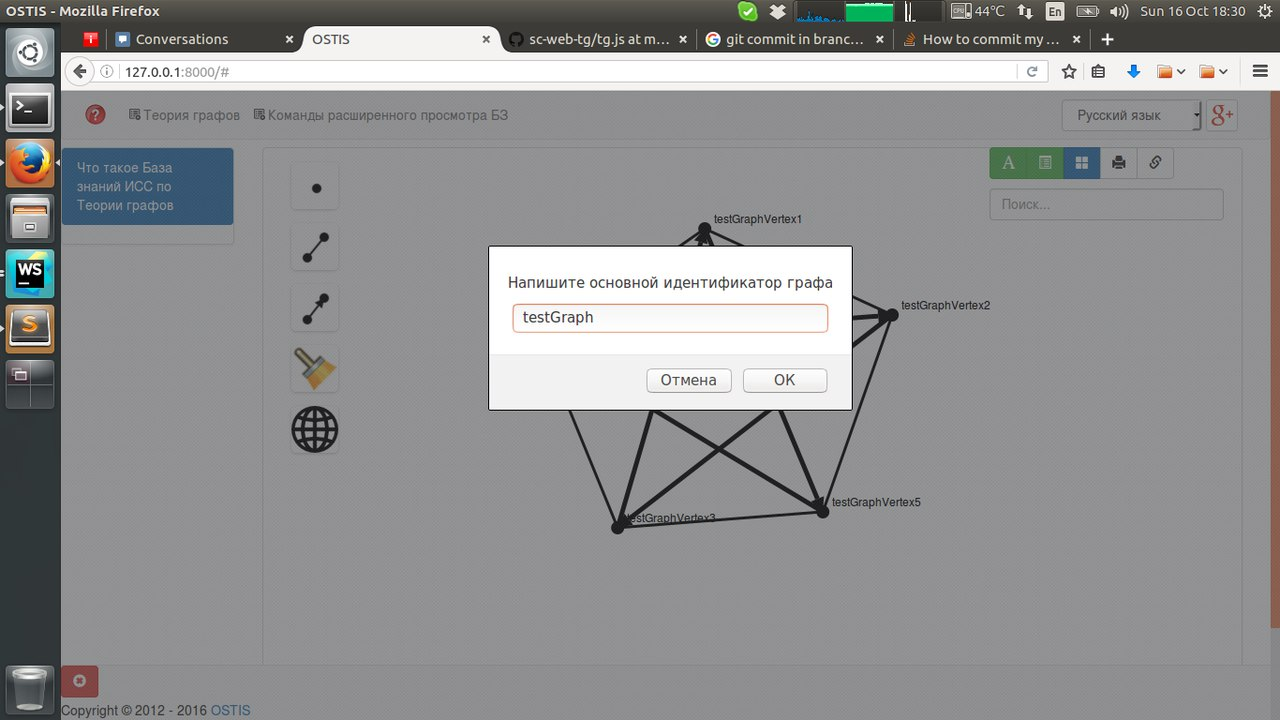
\includegraphics[width=\textwidth]{2.jpg}
  \caption{Окно для ввода основного sc-идентификатора}
  \label{fig:hardware:sdr_pipeline}
\end{figure}

\begin{figure}[H]
  \centering
  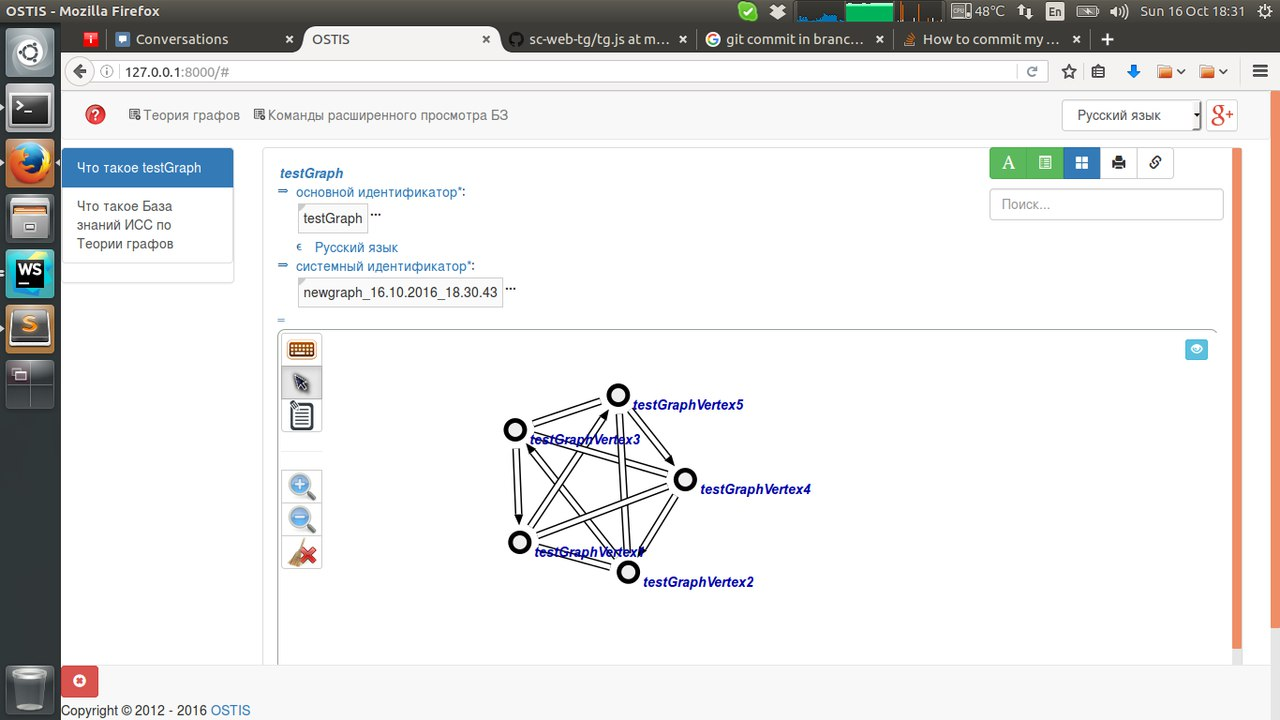
\includegraphics[width=\textwidth]{3.jpg}
  \caption{Семантическая окрестность нового графа}
  \label{fig:hardware:sdr_pipeline}
\end{figure}

\newpage
\subsection{Реализация компонента редактора графов}

В рамках этого пункта, на базе SCg-редактора был реализован собственный компонент для редактирования графов. Для этого были выполнены следующие задачи:

\begin{enumerate}
\item{Реализован скрипт установки редактора графов;}
\item{Написан скрипт сборки редактора графов;}
\item{Адаптирован SCg компонент под нужды редактор графов.}
\end{enumerate}

{\itshape
1) Реализован скрипт установки редактора графов.}

В рамках этой задачи, был изменен скрипт установки системы. Для этого был изменен файл prepare.sh и написан update\_component.sh и prepare\_web.sh

\begin{listing}[H]
  \begin{minted}{bash}
  
    ...
    base_path=../gt.ostis-Drawings/sc-web
    sc_web_path=../sc-web/client
    sc_web_static_path=$sc_web_path/static
    stage "Build component"
    cd $base_path
    python build_components.py -a -i
    cd -
    cp -r ../gt.ostis-Drawings/kb/graph_drawings/ ../kb/
    ...
    ./prepare_web.sh.
  \end{minted}
  \caption{Фрагмент файла update\_component.sh}
  \label{lst:practice:modelling_example}
\end{listing}

\begin{listing}[H]
  \begin{minted}{bash}
    ...
    cd ../sc-web/scripts
    ./prepare_js.sh
    python build_components.py -i -a
    ...
    cp -f ../config/server.conf ../sc-web/server/
  \end{minted}
  \caption{Фрагмент файла prepare\_web.sh}
  \label{lst:practice:modelling_example}
\end{listing}

\begin{listing}[H]
  \begin{minted}{bash}
    ...
    ./update_component.sh $st
    ...
  \end{minted}
  \caption{Фрагмент файла prepare.sh}
  \label{lst:practice:modelling_example}
\end{listing}

{\itshape
2) Написан скрипт сборки редактора графов.}

Для удобства разработки редактора и быстрой сборки, был написан набор скриптов для программы grunt. 

\begin{listing}[H]
  \begin{minted}{javascript}
    module.exports = function(grunt) {
        var tasks = require('./grunt_tasks.js')();
        grunt.initConfig(tasks);
        require('load-grunt-tasks')(grunt);
        grunt.registerTask('build', ['concat']);
        grunt.registerTask('default', ['concat', 'watch']);
    };
  \end{minted}
  \caption{Скрипт запуска сборки проекта }
  \label{lst:practice:modelling_example}
\end{listing}

Для сборки javascript файлов проекта необходимо выполнить команду grunt в терминале. Для обычных пользователей сборка проекта может осуществляться привычным им способом через python скрипт.

{\itshape
3) Адаптирован SCg компонент под нужды редактор графов.}

В рамках этой задачи, было изменено пространство имен SCg редактора на наше собственное. Это позволило использовать одновременно два редактора. Интерфейс нового компонента был адаптирован под необходимые функциональные возможности редактора графов. 

\begin{figure}[H]
  \centering
  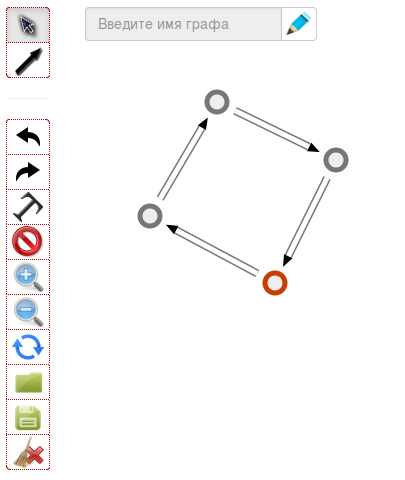
\includegraphics[scale=0.55]{5.png}
  \caption{Интерфейс редактора графов}
  \label{fig:hardware:sdr_pipeline}
\end{figure}

Реализован объект SCggKeynodesHandler. Данный объект предоставляет доступ к адресам sc-элементов, необходимых редактору графов.

\begin{listing}[H]
  \begin{minted}{javascript}
    SCggKeynodesHandler = {
        systemIds: [
            'format_scs_json',
            'nrel_gt_idtf',
            'nrel_weight',
            'nrel_temporal_decomposition',
            'rrel_current_version',
            'rrel_vertex',
            'rrel_oredge'
        ],
        scKeynodes: {},
        
        ...
    };
  \end{minted}
  \caption{Фрагмент объекта SCggKeynodesHandler}
  \label{lst:practice:modelling_example}
\end{listing}

Добавлена подписка компонента на события клавиатуры и обновления:

\begin{listing}[H]
  \begin{minted}{javascript}
    this.window_id = this.domContainer.substring(index) + '_' +
            this.sandbox.command_state.format;
    SCWeb.ui.KeyboardHandler.subscribeWindow
            (this.window_id, this.editor.keyboardCallbacks);
  \end{minted}
  \caption{Подписка компонента на события клавиатуры}
  \label{lst:practice:modelling_example}
\end{listing}

Изменен набор дуг и узлов.

\begin{figure}[H]
  \centering
  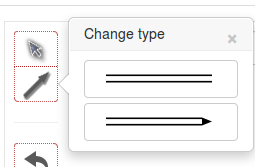
\includegraphics[scale=0.5]{6.png}
  \caption{Измененный набор дуг}
  \label{fig:hardware:sdr_pipeline}
\end{figure}

Написана спецификация к формату языка, редактору и его компонентам.

\newpage
\subsection{Реализация загрузки графа из SC-памяти в редактор графов}

В рамках этого задания, была реализована загрузка графа из sc-памяти в интерфейс редактора графов.

Чтобы загрузить граф в интерфейс, необходимо найти граф(главный узел графа с темпоральной декомпозицией или узел-структуру) и открыть редактор.

\begin{figure}[H]
  \centering
  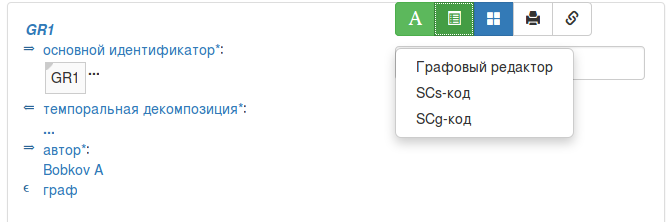
\includegraphics[scale=0.70]{7.png}
  \caption{Страница с графом перед открытием в редакторе}
  \label{fig:hardware:sdr_pipeline}
\end{figure}

Также этот граф можно открыть со страницы семантической области графа без темпоральной декомпозиции

\begin{figure}[H]
  \centering
  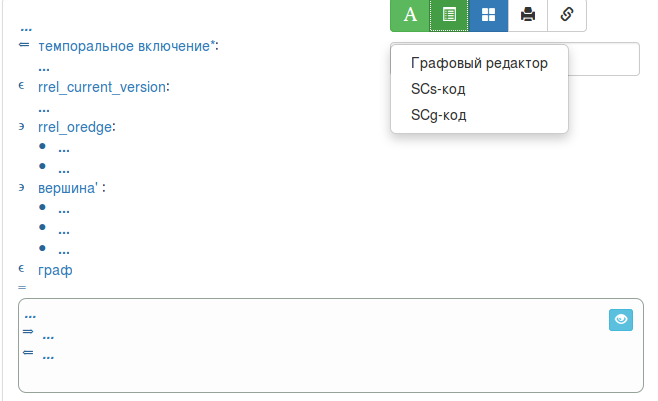
\includegraphics[scale=0.70]{8.png}
  \caption{Страница с графом перед открытием в редакторе}
  \label{fig:hardware:sdr_pipeline}
\end{figure}

Открытие осуществляется через элемент смены внешнего языка для активного окна.

\begin{figure}[H]
  \centering
  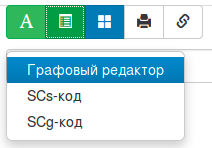
\includegraphics[scale=0.65]{9.png}
  \caption{Открыть граф в редакторе графов}
  \label{fig:hardware:sdr_pipeline}
\end{figure}

Если активное окно пользователя содержало граф, будет предложен выбор об открытии графа или создании нового. Если пользователь открыл редактор графов в окне, где не было графа или нажал на кнопку «Новый граф», будет открыт пустой редактор, в котором можно будет создать новый граф.

\begin{figure}[H]
  \centering
  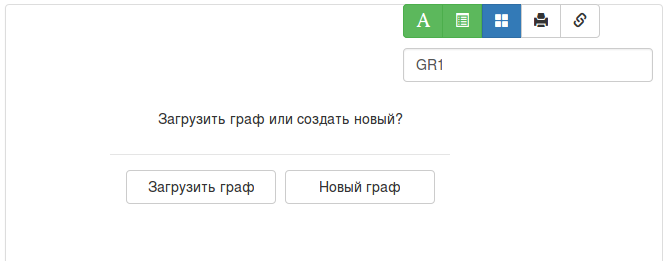
\includegraphics[scale=0.65]{10.png}
  \caption{Форма выбора}
  \label{fig:hardware:sdr_pipeline}
\end{figure}

Спецификация формы была добавлена в базу знаний. Это позволила изменять форму в зависимости от выбранного языка.

\begin{figure}[H]
  \centering
  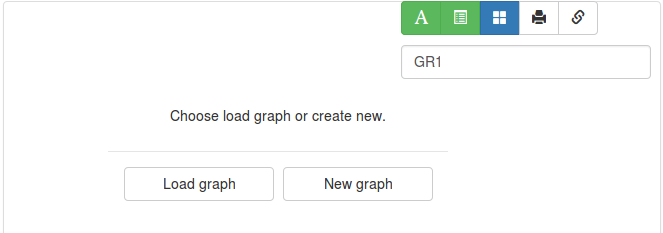
\includegraphics[scale=0.65]{11.png}
  \caption{Форма выбора}
  \label{fig:hardware:sdr_pipeline}
\end{figure}

Если пользователь нажал открыть граф, то он появится в редакторе.

\begin{figure}[H]
  \centering
  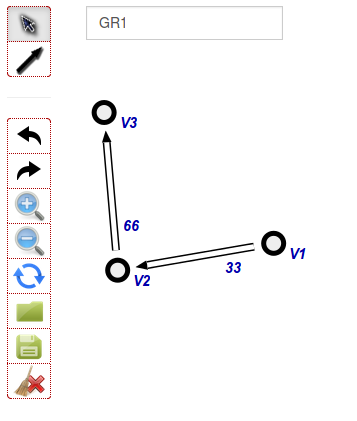
\includegraphics[scale=0.75]{12.png}
  \caption{Граф в редакторе}
  \label{fig:hardware:sdr_pipeline}
\end{figure}

К вершинам графа будут подгружены их идентификаторы, а к ребрам их вес.

\newpage
\subsection{Встраивание SCs-компонента в редактор}

Для быстрого осмотра семантической окрестности элементов графа в редактор графов был встроен SCs компонент. В него автоматически загружается семантическая окрестность выделенного элемента, если он находится в памяти. Если ни один элемент графа не выделен, загружается полная семантическая окрестность самого графа.

На данный момент семантические окрестности выглядят следующим образом:

\begin{figure}[H]
  \centering
  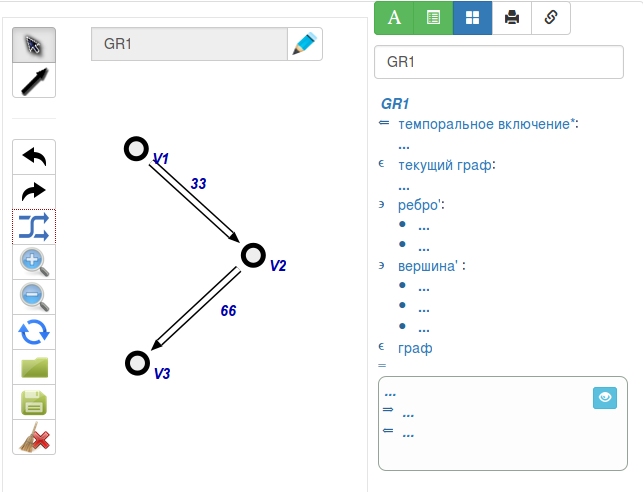
\includegraphics[scale=0.75]{13.png}
  \caption{Семантическая окрестность графа(ничего не выделено)}
  \label{fig:hardware:sdr_pipeline}
\end{figure}

\begin{figure}[H]
  \centering
  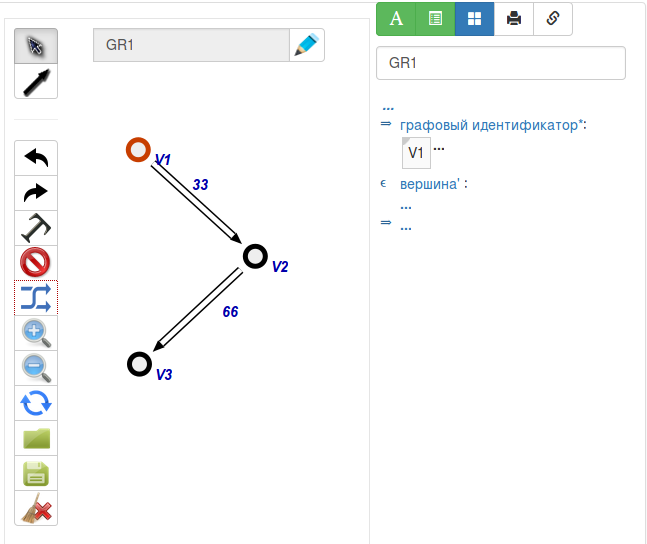
\includegraphics[scale=0.5]{14.png}
  \caption{Семантическая окрестность вершины графа}
  \label{fig:hardware:sdr_pipeline}
\end{figure}

\begin{figure}[H]
  \centering
  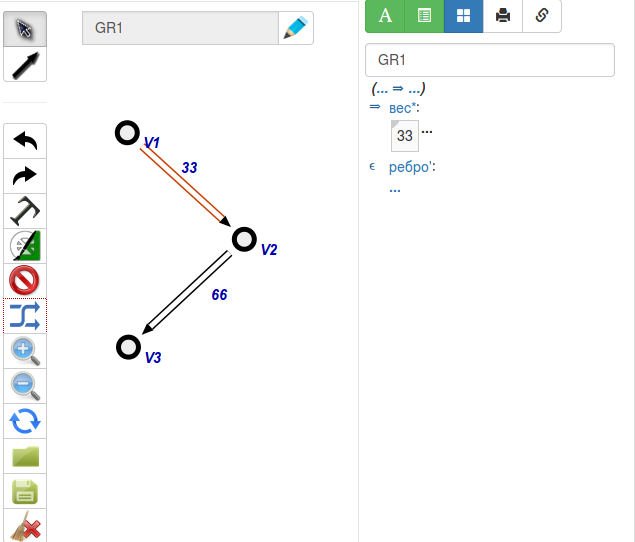
\includegraphics[scale=0.5]{15.png}
  \caption{Семантическая окрестность дуги графа}
  \label{fig:hardware:sdr_pipeline}
\end{figure}


В будущем, с целью повышения наглядности, планируется заменить агент поиска полной семантической окрестности элемента на свои агенты, выводящие только необходимую для пользователя информацию.

\newpage
\subsection{Интегрирование решателя задач в редактор графов}

Мною был интегрирован компонент для вызова решателя задач для текущего графа в редакторе.

\begin{figure}[H]
  \centering
  
\includegraphics[scale=0.75]{16.png}
  \caption{Компонент решения задачи}
  \label{fig:hardware:sdr_pipeline}
\end{figure}

При нажатии на поле «Выбор условия», появляется всплывающее окно с вводом условия.

\begin{figure}[H]
  \centering
  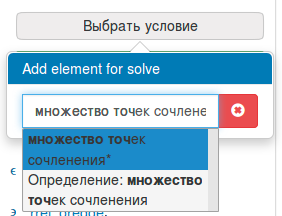
\includegraphics[scale=0.75]{17.png}
  \caption{Выбор решаемой задачи}
  \label{fig:hardware:sdr_pipeline}
\end{figure}

При нажатии на кнопку «Решение задачи», в историю добавляется новое окно с деревом решения задачи. В редакторе обновляется SCn-компонент.

\begin{figure}[H]
  \centering
  
\includegraphics[scale=0.5]{18.png}
  \caption{Добавление и отображение решения в историю}
  \label{fig:hardware:sdr_pipeline}
\end{figure}

\begin{figure}[H]
  \centering
  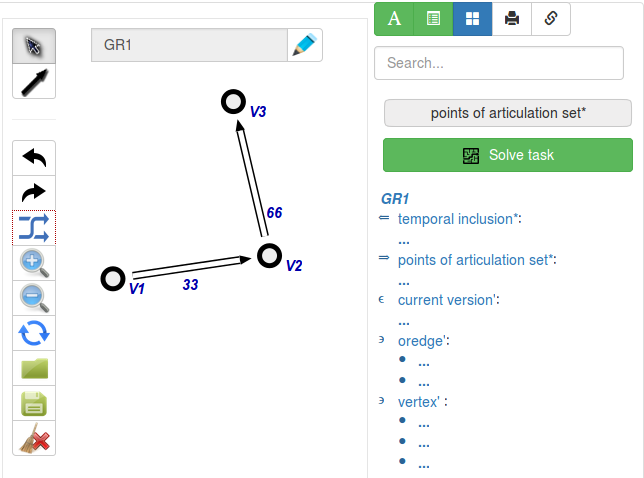
\includegraphics[scale=0.75]{19.png}
  \caption{Обновление SCn компонента}
  \label{fig:hardware:sdr_pipeline}
\end{figure}


\subsection{Помощь другим участникам}

Мною была осуществлена работа по курированию репозитория с редактором графов. В ходе этой работы было произведено:

\begin{enumerate}
\item{Рассказано про возможности SCg редактора и основы ядра пользовательского интерфейса;}
\item{Осуществлена помощь с решением поставленных задач;}
\item{Произведено тестирование и просмотр кода других участников.}
\end{enumerate}


\newpage
\section{Личный вклад в развитие проекта по SCg-интерфейсу}
\label{sec:domain3}

\subsection{Генератор gwf файлов}

В рамках этой задачи мною были выполнены следующие задачи:
\begin{itemize}
\item{Добавлена библиотека для создания файлов;}
\item{Создан объект для сохранения файлов;}
\item{Добавлена кнопка сохранения файла и ее спецификация в БЗ;}
\item{Исправлены проблемы с неправильным названием дуг;}
\item{Исправлена модель шины для корректного сохранения файла.}
\end{itemize}

\begin{figure}[H]
  \centering
  
\includegraphics[scale=1]{20.png}
  \caption{Кнопка создания gwf файла}
  \label{fig:hardware:sdr_pipeline}
\end{figure}

\begin{figure}[H]
  \centering
  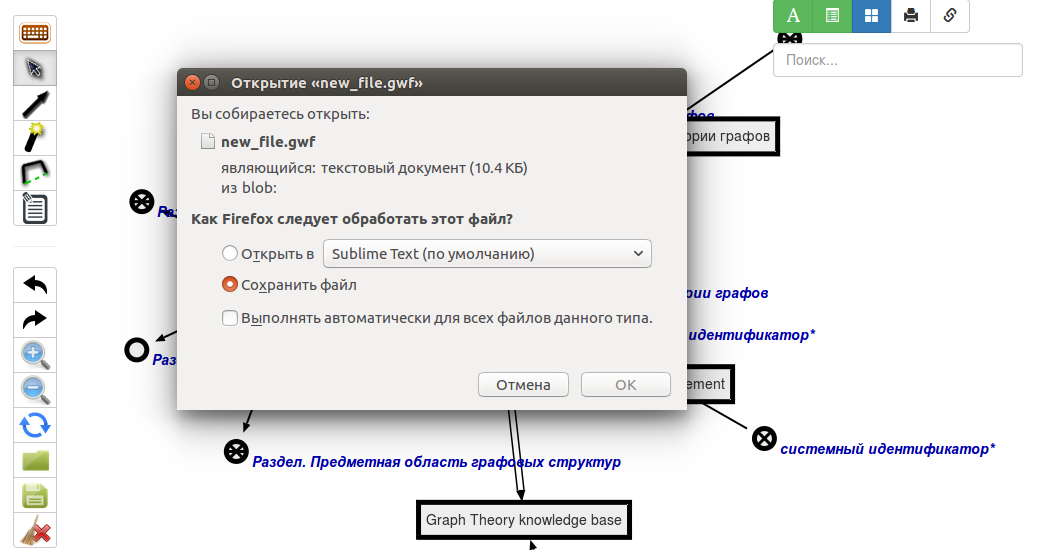
\includegraphics[width=\textwidth]{21.png}
  \caption{Окно сохранения файла}
  \label{fig:hardware:sdr_pipeline}
\end{figure}

\begin{figure}[H]
  \centering
  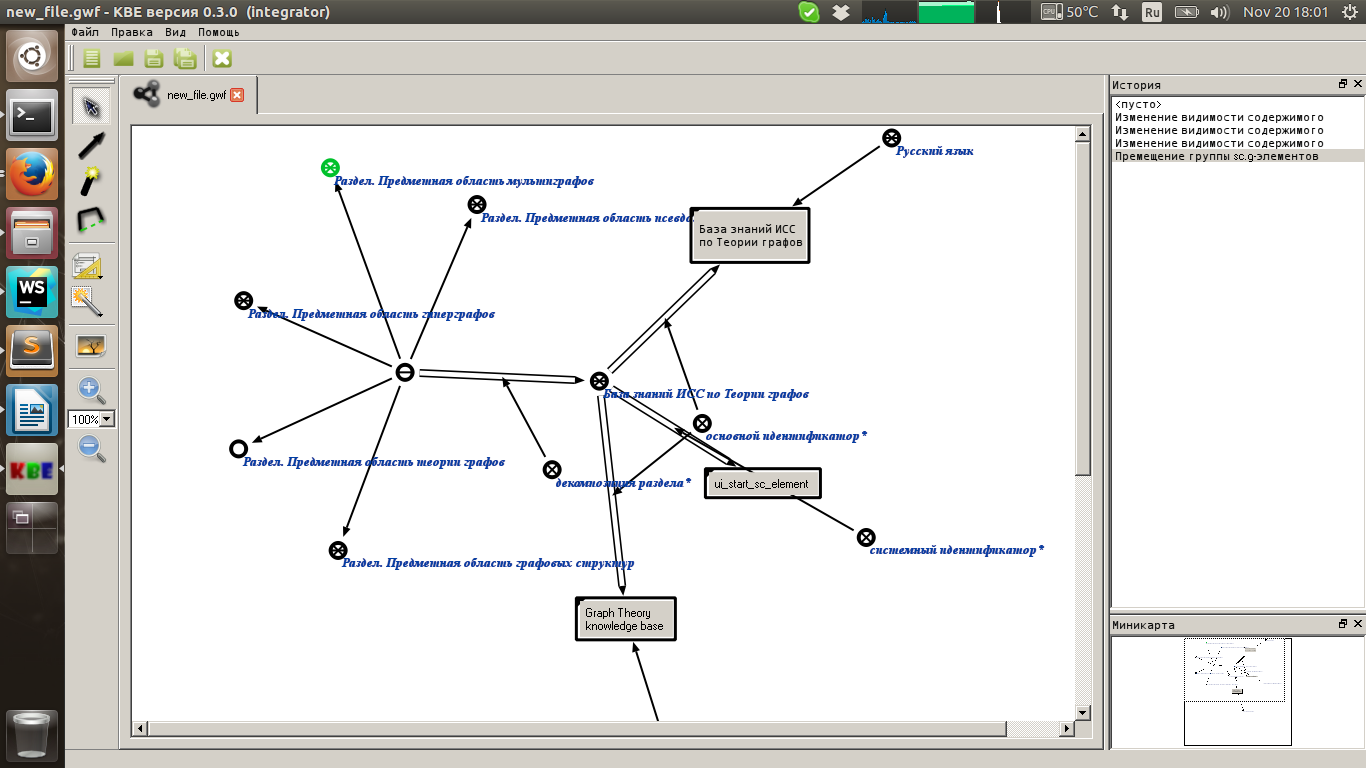
\includegraphics[width=\textwidth]{22.png}
  \caption{Открытие файла в KBE}
  \label{fig:hardware:sdr_pipeline}
\end{figure}

Для создания gwf файла был написан объект GwfFileCreate и 18 необходимых для его работы функции.

\begin{listing}[H]
  \begin{minted}{javascript}
GwfFileCreate = {
    scene: null,
    fileString: null,
    createFile: function (scene) {
        this.scene = scene;
        this.fileString = "";
        var self = this;
        this.addHeaderFile();
        ...
        this.scene.edges.forEach(function (edge) {
            self.createEdge(edge);
        });
        this.addEndFile();
        return this.fileString;
    },
    ...
}
  \end{minted}
  \caption{Фрагмент объекта GwfFileCreate}
  \label{lst:practice:modelling_example}
\end{listing}

\newpage
\subsection{Создание подписки компонентов}

В рамках этой задачи был создан объект OpenComponentHandler, который подписывает компоненты и вызывает функцию компонента openComponentCallbacks при открытии компонента в браузере. Данный объект помог решить проблему неправильного отображения элементов после просмотра других компонентов.

\begin{listing}[H]
  \begin{minted}{javascript}
SCWeb.ui.OpenComponentHandler = {
    events: {},
    subscribeComponent: function (windowId, callback) {
        this.events[windowId] = callback;
    },
    unsubscribeComponent: function (windowId) {
        delete this.events[windowId];
    },
    callOpenComponentCallback: function (windowId) {
        if (this.events.hasOwnProperty(windowId)){
            this.events[windowId]();
        }
    }
};
  \end{minted}
  \caption{Фрагмент объекта OpenComponentHandler}
  \label{lst:practice:modelling_example}
\end{listing}


\begin{listing}[H]
  \begin{minted}{javascript}
if(component.editor){
    ...
    if(component.editor.openComponentCallbacks) {
        SCWeb.ui.OpenComponentHandler.subscribeComponent(
            options.window_id,
            component.editor.openComponentCallbacks
        );
    }
}
  \end{minted}
  \caption{Пример подписки SCg-компонента}
  \label{lst:practice:modelling_example}
\end{listing}

\newpage
\subsection{Загрузка изображений в память}

Добавлена возможность вставлять в ссылку файлы изображения. Для корректного отображения изображений и обеспечения совместимости SCg-редактора с KBE редактором, был переделан компонент вывода изображений ImageComponent.

\begin{figure}[H]
  \centering
  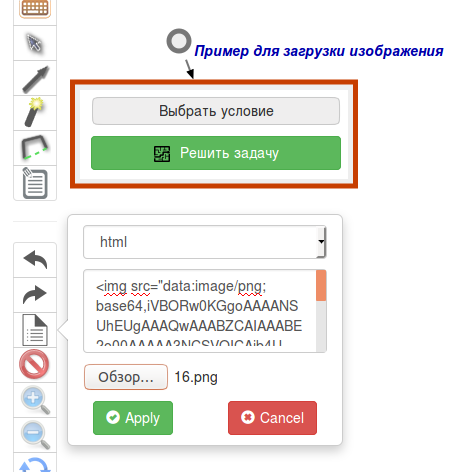
\includegraphics[scale=0.75]{24.png}
  \caption{Загрузка изображения в SCg-редакторе}
  \label{fig:hardware:sdr_pipeline}
\end{figure}

\begin{figure}[H]
  \centering
  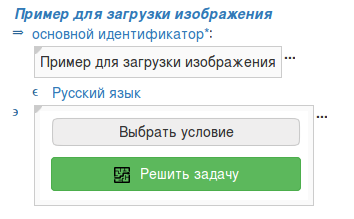
\includegraphics[scale=0.75]{25.png}
  \caption{Результат трансляции изображения}
  \label{fig:hardware:sdr_pipeline}
\end{figure}

\newpage
\subsection{Другая работа по SCg-редактору}
1) Были уменьшены размеры кнопок для более удобного отображения элементов редактора у пользователей с небольшим разрешением монитора.

2) Была исправлена проблема с отображением ссылок, при переключении на другую страницу в истории.

3) Исправлена проблема c невозможностью создания элементов после удаления всех элементов. 

4) Реализована кнопка очистки всех объектов с рабочей области редактора и написана ее спецификация.

\begin{figure}[H]
  \centering
  
\includegraphics[scale=0.75]{tool-clear.png}
  \caption{Кнопка очистки всех элементов}
  \label{fig:hardware:sdr_pipeline}
\end{figure}

5) Исправлены опечатки в коде(орфографические ошибки и неправильные названия в переменных и объектах.

6) Добавлена возможность загружать в ссылки html текст и html файлы.

\begin{figure}[H]
  \centering
  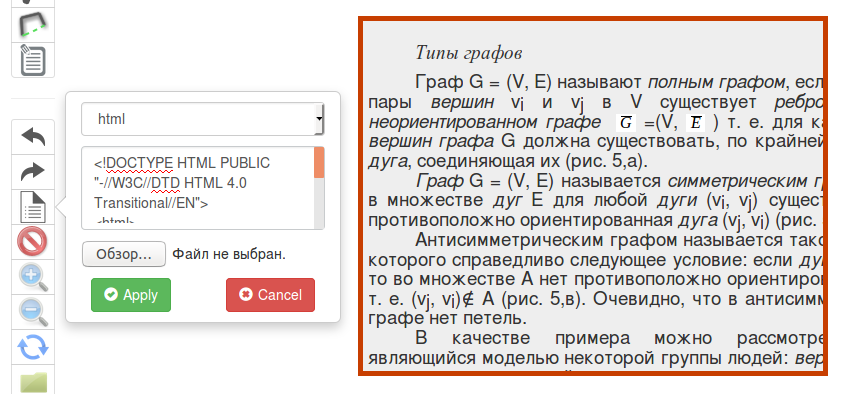
\includegraphics[width=\textwidth]{23.png}
  \caption{Иконка кнопки очистки всех элементов}
  \label{fig:hardware:sdr_pipeline}
\end{figure}

7) Удалены неиспользуемые файлы javascript.

8) Исправлена неправильная подписка компонентов.

9) Начата работа по отображению SCg файлов в ссылках SCn-статей.
Для этого был создан объект и добавлен необходимый функционал в SCg-компонент.

На данный момент компонент отображается только в  SCn-комопоненте и не работает в SCg-компоненте из-за проблемы рекурсивного использования компонента.

\begin{figure}[H]
  \centering
  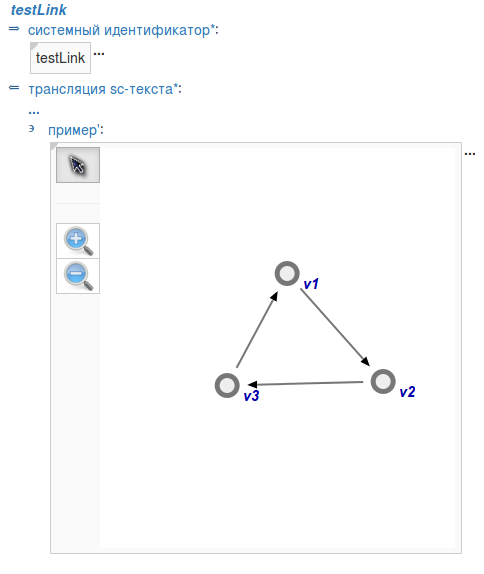
\includegraphics[scale=0.75]{lik_GFW.png}
  \caption{Пример отображения gwf фала в ссылке}
  \label{fig:hardware:sdr_pipeline}
\end{figure}

\newpage
\section{Личный вклад в развитие проекта по SCn-интерфейсу}
\label{sec:domain4}

\subsection{Реализация редактора ссылок}

В рамках этой задачи был реализован редактор ссылок. Редактор позволяет создавать новые ссылки или редактировать текущий ссылки. Для создания или редактирования ссылки необходимо выделить нужный узел или ссылку и нажать кнопку «->ссылка»

\begin{figure}[H]
  \centering
  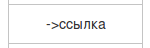
\includegraphics[scale=1]{28.png}
  \caption{Кнопка для редактирования ссылок}
  \label{fig:hardware:sdr_pipeline}
\end{figure}

\begin{figure}[H]
  \centering
  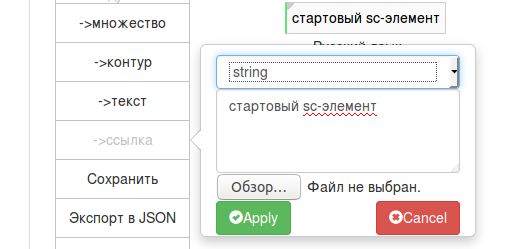
\includegraphics[scale=0.5]{29.png}
  \caption{Внешний вид редактора ссылок}
  \label{fig:hardware:sdr_pipeline}
\end{figure}

Пример редактирования изображения:

\begin{figure}[H]
  \centering
  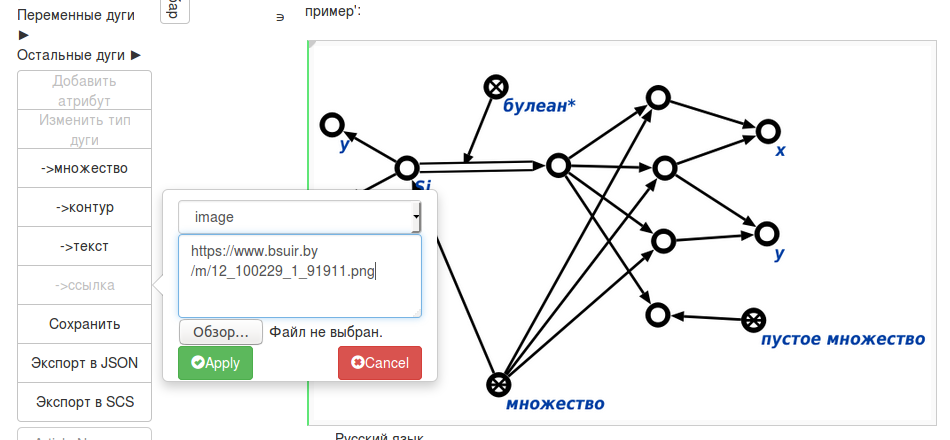
\includegraphics[scale=0.4]{31.png}
  \caption{Редактирование картинки в ссылке}
  \label{fig:hardware:sdr_pipeline}
\end{figure}


\begin{figure}[H]
  \centering
  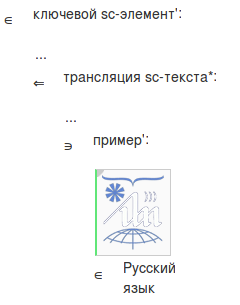
\includegraphics[scale=1]{32.png}
  \caption{Новая картинка в ссылке}
  \label{fig:hardware:sdr_pipeline}
\end{figure}


Редактор поддерживает следующие форматы для редактирования:
\begin{itemize}
\item{string;}
\item{html;}
\item{image;}
\item{youtube;}
\item{googlemap;}
\item{video.}
\end{itemize}

Реализована загрузка html файлов и изображений в ссылку.

\newpage
\subsection{Создание нескольких SCn-статей в рамках контура}

Была решена проблема создания нескольких SCn-статей в рамках одного контура. Для реализации этой задачи было исправлено выделения элементов, написаны команды для вставки и удаления статьи, исправлена модель контура и транслирование элементов контура в память.

Добавление SCn-статьи в контур происходит путем выделения контура или первой SCn-статьи в контуре и нажатием на кнопку «->контур»

\begin{figure}[H]
  \centering
  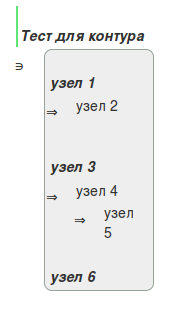
\includegraphics[scale=0.6]{33.png}
  \caption{Новая картинка в ссылке}
  \label{fig:hardware:sdr_pipeline}
\end{figure}

\begin{figure}[H]
  \centering
  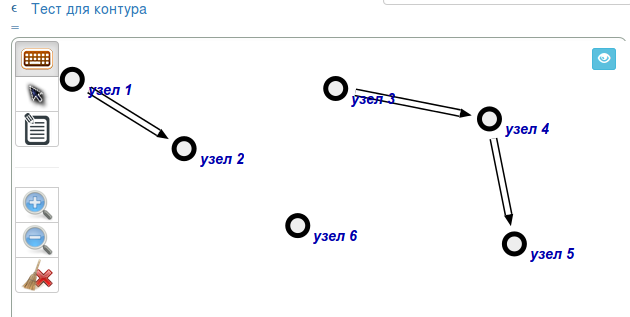
\includegraphics[width=\textwidth]{34.png}
  \caption{Результат транслирования}
  \label{fig:hardware:sdr_pipeline}
\end{figure}

\newpage
\subsection{Реализация правил для редактирования основных идентификаторов}

В рамках этой задачи, мною была реализована логика для изменения основного идентификатора узла согласно следующим правилам:

1) Можно редактировать идентификатор корневого элемента статьи, в таком случае он изменится во всей базе знаний

2) Можно редактировать содержимое любой sc-ссылки. Если она является идентификатором некоторого элемента, то он изменится во всей базе знаний

3) Запрещено редактировать идентификаторы любых элементов статьи, не являющихся корневыми, за исключением случая, когда создан новый элемент с идентификатором, который ранее не существовал в базе. В случае, когда при редактировании происходит обращение к уже существующему идентификатору, то элемент редактируемой статьи "склеивается" с существующим в базе и редактировать его имя запрещено. При необходимости изменений должна удаляться и создаваться заново минимально необходимая конструкция

\begin{figure}[H]
  \centering
  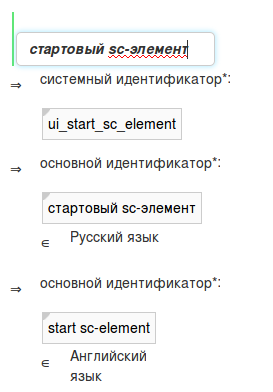
\includegraphics[scale=0.75]{35.png}
  \caption{Редактирование корневого элемента}
  \label{fig:hardware:sdr_pipeline}
\end{figure}

\newpage
\subsection{Другая работа по SCn-редактору}
1) Исправлена проблема с обновлением корневого элемента контура.

2) Исправлена проблема с отображением html файлов в ссылках.

\begin{figure}[H]
  \centering
  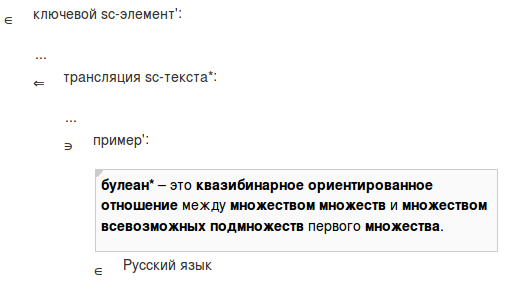
\includegraphics[scale=0.75]{26.png}
  \caption{Пример отображения html файла в ссылке}
  \label{fig:hardware:sdr_pipeline}
\end{figure}

3) Исправлена проблема с невозможность открыть SCg-редактор в SCn-статье. 

\begin{figure}[H]
  \centering
  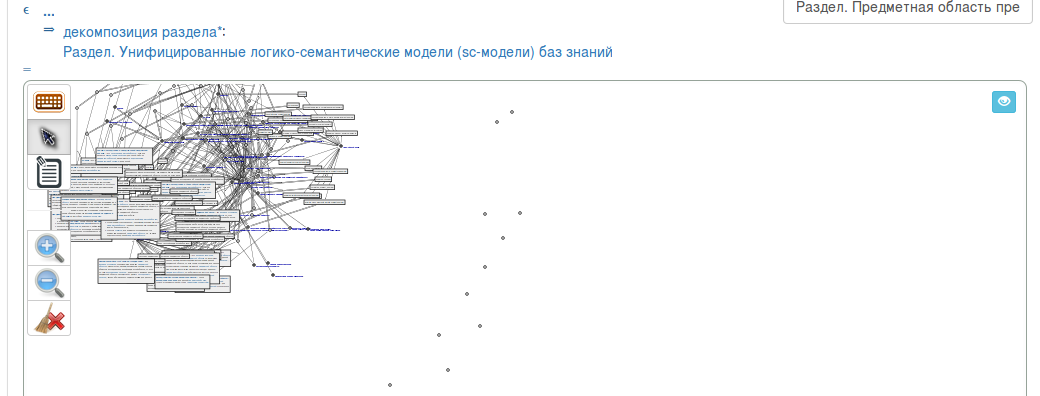
\includegraphics[scale=0.40]{27.png}
  \caption{Пример открытого SCg-редактора в SCn-статье}
  \label{fig:hardware:sdr_pipeline}
\end{figure}

4) Исправлено снятие выделения элементов в редактор. 

5) Произведено тестирование компонента, в результате которого найдено более шести проблем.

\newpage
\section{Направления дальнейшего развития разработанных системы}
\label{sec:domain5}

В следующем семестре я планирую продолжить работу над развитием SCg-редактора и SCn-редактора. Устранить существующие недоработки, добавить туда новые функции.

Для проекта ИСС по Теории Графов в следующем семестре я планирую:
\begin{itemize}
\item{Совершенствовать отображение графов;}
\item{Совершенствовать редактор графов.}
\end{itemize}




